\documentclass[11pt,a4paper,oneside]{book}
\usepackage[margin=21mm,headheight=16pt]{geometry}
\usepackage{fontspec}
\setmainfont{Noto Sans}
\newfontfamily\displayfont{EB Garamond}
\usepackage{xcolor,graphicx,enumitem,tabularx,booktabs,titlesec,fancyhdr,microtype}
\usepackage[most]{tcolorbox}
\usepackage{pdfpages}
\usepackage{hyperref}
\definecolor{paper}{HTML}{FFFDFA}
\definecolor{ink}{HTML}{2A354B}
\definecolor{navy}{HTML}{08142C}
\definecolor{blue}{HTML}{274B75}
\definecolor{rule}{HTML}{E1DACA}
\pagecolor{paper}\color{ink}
\hypersetup{colorlinks=true,urlcolor=blue,linkcolor=blue,pdftitle={The Future Is Written — English C},pdfauthor={}}
\setlength{\parindent}{0pt}
\setlength{\parskip}{.55em}
\linespread{1.12}
\setlist{leftmargin=*,itemsep=.35em,topsep=.4em,parsep=0pt}
\setlist[enumerate]{label=\textcolor{blue}{\arabic*.}}
\titleformat{\section}{\displayfont\Large\color{navy}}{}{0pt}{}
\titlespacing*{\section}{0pt}{1.2em}{.5em}
\newcommand{\tasktitle}[1]{{\color{blue}\bfseries #1}\par\smallskip}
\newtcolorbox{taskbox}{enhanced,colback=paper,colframe=paper,boxrule=0pt,left=3mm,right=1mm,top=1mm,bottom=1mm,before skip=5pt,after skip=8pt}
\newtcolorbox{quotebox}{enhanced,breakable,colback=paper,colframe=rule,boxrule=0pt,borderline west={2pt}{0pt}{rule},fontupper=\displayfont\large,left=5mm}
\pagestyle{fancy}\fancyhf{}
\fancyhead[L]{\small\color{blue}The Future Is Written}
\fancyhead[R]{\small English C}
\fancyfoot[L]{\footnotesize\nouppercase{\leftmark}}
\fancyfoot[R]{\small\thepage}
\renewcommand{\headrulewidth}{0pt}
\setcounter{tocdepth}{0}
\begin{document}
\begin{titlepage}
\vspace*{12mm}
{\color{blue}\large ENGLISH C\par}
\vspace{8mm}
{\displayfont\color{navy}\fontsize{43}{47}\selectfont The Future\\Is Written\par}
\vspace{12mm}
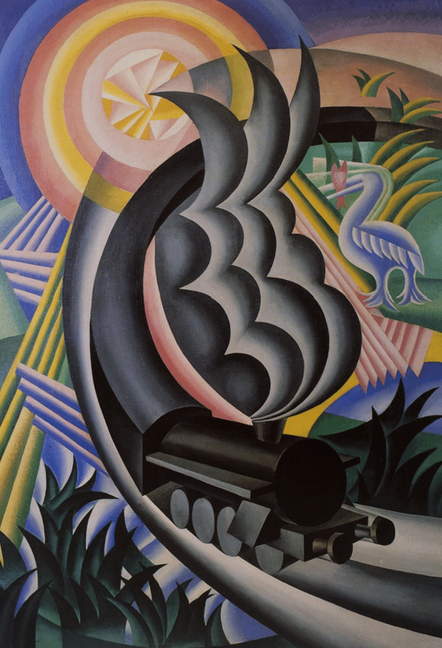
\includegraphics[width=\linewidth,height=.48\textheight,keepaspectratio]{assets/Sci-fi-train.png}
\vfill
{\large Science fiction, memory, artificial intelligence,\\human relationships, and space exploration.\par}
\vspace{5mm}
{\color{blue}Nine lessons · 19 October–23 November 2026\par}
\end{titlepage}
\tableofcontents
\clearpage

\clearpage\markboth{Brave New World}{}
\addcontentsline{toc}{chapter}{1. Brave New World}
{\color{blue}\small LESSON 01 \hfill 19 October 2026\par}
\vspace{4mm}
{\displayfont\color{navy}\fontsize{30}{34}\selectfont Brave New World\par}\vspace{4mm}

\section*{Program}

\begin{itemize}
\item \emph{12.05} Warm up
\item \emph{12.15} Utopias and dystopias
\item \emph{12.45} Break
\item \emph{13.00} Types of sci-fi
\item \emph{13.15} Brave New World
\item \emph{14.00} Break
\item \emph{14.10} Reading
\end{itemize}

\section*{Warm up}
\begin{quotebox}
people will come to love their oppression, adore the technologies that undo their capacities to think.

— Aldous Huxley

\end{quotebox}
\begin{taskbox}
\tasktitle{Discuss with your classmates}
\begin{enumerate}
\item Are you mainly optimistic or pessimistic about the future?
\item What role does technology/science play in your vision of the future?
\item Discuss Aldous Huxley’s quote above. To what extent do you agree/disagree?
\end{enumerate}
\end{taskbox}

\section*{Utopias and dystopias}
As the thought experiments above indicate, there are basically two kinds of science fiction: utopian and dystopian. The word 'utopia' was coined by the British writer Thomas More in 1516. Utopia, meaning 'good place',was the title of his book which outlined a perfect, flawless and harmonious society without any greed, corruption or power struggles due to the fact that there was no private property. The opposite of a utopia is dystopia. Like 'utopia', the word has Greek roots and simply means 'bad place', in other words a worst-case scenario of how a society might turn out.


\begin{itemize}
\item \emph{Topos}: Greek for “place”.
\item \emph{Ou}: Greek for “not” or “no”.
\item \emph{Eu}: Greek for “good” or “well”.
\item \emph{Dys}: Greek for “bad” or “difficult”.
\end{itemize}
\begin{taskbox}
\tasktitle{Draw in pairs}
\begin{enumerate}
\item Instruct your classmate to draw a place that you think could be called u-/dystopia.
\end{enumerate}
\end{taskbox}

\section*{Types of sci-fi}
Earlier, we learned that there are basically two kinds of science fiction: utopian and dystopian. There are, however, also a few other sets of pairs that might help us understand what sci-fi is. The first one is that there are sci-fi stories set in outer space, commonly known as ‘space operas’, as well as sci-fi stories set on Earth in a more or less distant future, for instance Brave New World and Nineteen Eighty-Four that we mentioned above. Space opera with aliens, spaceships, galactic wars, cyborgs and so on is perhaps the least respected of the sub-genres of science fiction, but also one of the most popular and certainly what most people associate with science fiction.

Secondly, there are also two kinds of sci-fi stories in the sense that there is ‘hard science fiction’ and ‘soft science fiction’. Soft science fiction is used to describe stories that focus on the human element rather than scientific facts and technical details. Hard SF, on the other hand, is the most science-oriented category and focuses on facts. Hard SF is also more likely to use the language of science directly. Since this type of SF sticks to facts, it usually explores what already exists, i.e. the perspectives already opened up by contemporary science and technology. However, the boundaries between the two kinds might be blurred and to some extent the categories are marketing terms used to target different groups of readers.


\begin{tabularx}{\linewidth}{@{}XX@{}}\toprule
Types - in terms of opposites & \\
utopian & dystopian\\
space stories, incl. space operas & future on earth stories\\
hard sci-fi & soft sci-fi\\
near future & far future\\
\bottomrule\end{tabularx}\par\medskip
\begin{taskbox}
\tasktitle{Discuss}
\begin{enumerate}
\item Have you read or watched stories that fit either of the categories?
\end{enumerate}
\end{taskbox}

\section*{Brave New World}

\noindent\begin{minipage}[c]{.51\linewidth}
\begin{quote}\tasktitle{Work with the text}

\begin{enumerate}
\item Do the exercises on the handout.
\item Read the first chapter of Brave New World
\end{enumerate}
\end{quote}
\end{minipage}\hfill\begin{minipage}[c]{.44\linewidth}\centering
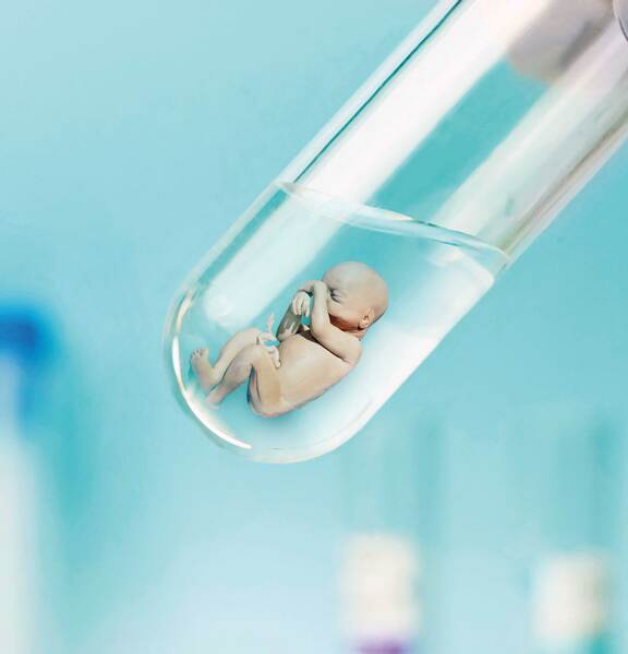
\includegraphics[width=\linewidth,height=.4\textheight,keepaspectratio]{assets/1792400829-bnw.png}\end{minipage}\par\medskip

\section*{Materials}

\begin{itemize}
\item \hyperref[worksheet-1]{Brave New World: Worksheet (p.~\pageref*{worksheet-1})}
\item Brave New World: Excerpt
\end{itemize}

\clearpage\markboth{Brave New World II}{}
\addcontentsline{toc}{chapter}{2. Brave New World II}
{\color{blue}\small LESSON 02 \hfill 22 October 2026\par}
\vspace{4mm}
{\displayfont\color{navy}\fontsize{30}{34}\selectfont Brave New World II\par}\vspace{4mm}

\section*{Program}

\begin{itemize}
\item \emph{08.35} Warm up / recap
\item \emph{09.05} World building
\item \emph{09.25} Break
\item \emph{09.40} Analysis
\item \emph{10.30} Break
\item \emph{10.40} Adaptation
\end{itemize}

\section*{Warm up / recap}
\begin{taskbox}
\tasktitle{In pairs:}
\begin{enumerate}
\item Make a list of the casts of this society, and the jobs reserved for the members of these casts.
\item One student is an Alpha from the Hatchery, the other an Epsilon. The Alpha student outlines the scientific advances and explain the Bokanovsky process so an Epsilon can understand it, and the Epsilon asks questions for clarification.
\end{enumerate}
\end{taskbox}
\begin{taskbox}
\tasktitle{Individually:}
\begin{enumerate}
\item Finish reading the first chapter of Brave New World
\item Make a list of the casts of this society, and the jobs reserved for the members of these casts.
\item Write an explanation of the Bokanovsky Process addressed to an Epsilon – simplify the scientific explanation so the Epsilon can understand you but stay true to the facts. Use informal English and be as objective as possible.
\end{enumerate}
\end{taskbox}

\section*{World building}
\begin{quotebox}
A squat grey building of only thirty-four stories. Over the main entrance the words, CENTRAL LONDON HATCHERY AND CONDITIONING CENTRE, and, in a shield, the World State’s motto, COMMUNITY, IDENTITY, STABILITY.

\end{quotebox}
In science fiction, the setting is often a character in itself. The above quote is however the only description of the outside world we get in the first chapter. What we get instead is a description of how society is structured. Can we use this to imagine how such a society might look?

\begin{taskbox}
\tasktitle{Create}
\begin{enumerate}
\item In the form of a poster (it may be digital), or a literary discription, make a depiction of the outside world of Brave New World.
\item Find five quotes that inspired your choices.
\end{enumerate}
\end{taskbox}

\section*{Analysis}
\begin{taskbox}
\tasktitle{Work with the text}
\begin{enumerate}
\item Discuss answers to the questions on the handout. Write down notes to your answers.
\end{enumerate}
\end{taskbox}

\section*{Adaptation}
Watch the first 18 minutes of the tv-show Brave New World and do the reflection exercise below

In the novel, the world state motto is "Community, Identity, Stability", in the show New London has three rules: "No privacy. No family. No monogamy".

\begin{taskbox}
\tasktitle{Reflect}
\begin{enumerate}
\item Write for 5 minutes about the the show's interpretation of the brave new world of the novel. Did the world look like you had imagined it? What's the connection between the New London rules and the World State motto?
\end{enumerate}
\end{taskbox}

\section*{Glossary}

\begin{itemize}
\item \textbf{Cognitive estrangement:} Science fiction makes familiar things seem strange so we can look at our own world in a new way. Its unfamiliar world follows an understandable logic.
\item \textbf{Info-dump:} A passage that gives the reader a large amount of background information about the fictional world at once. This can happen through a narrator’s explanation or a character’s speech, such as the Director’s tour of the Hatchery.
\end{itemize}

\section*{Materials}

\begin{itemize}
\item \hyperref[worksheet-2]{Brave New World: Handout (p.~\pageref*{worksheet-2})}
\item Brave New World: S01E01
\end{itemize}

\clearpage\markboth{The Relive Box}{}
\addcontentsline{toc}{chapter}{3. The Relive Box}
{\color{blue}\small LESSON 03 \hfill 26 October 2026\par}
\vspace{4mm}
{\displayfont\color{navy}\fontsize{30}{34}\selectfont The Relive Box\par}\vspace{4mm}

\section*{Program}

\begin{itemize}
\item \emph{12.05} Memory
\item \emph{12.25} Reading
\item \emph{12.55} Break
\item \emph{13.10} Reading - cont.
\item \emph{13.40} Formal vs. informal language
\item \emph{14.00} Working with the text
\item \emph{14.30} Summing up
\end{itemize}

\section*{Memory}
\begin{taskbox}
\tasktitle{vocabulary}
\begin{enumerate}
\item The words and expressions below are all related to memory. Look up the ones you are not familiar with.
\end{enumerate}
\emph{recollect – call to mind – a trip down memory lane – fix in the mind – hold dear – dwell on the past – recall – relive – think back – in retrospect – reminiscence – treasure – cherish – have a flashback – ring a bell – anamnesis – dig into the past – backtrace}

\end{taskbox}

\par\medskip{\color{rule}\hrule}\medskip
\begin{taskbox}
\tasktitle{In pairs}
2. How many of the words and expressions from previous slide can you remember?
3. If you had the chance to relive a memory from your past, what would it be and why? Describe the memory, what happens, the mood, the setting etc. You may include some of the words from the list in the previous slide.

\end{taskbox}

\par\medskip{\color{rule}\hrule}\medskip

\par\noindent\textbf{Video:} Spatial Scene is INSANE (Apple Vision Pro, visionOS 26)\par\medskip

\section*{Reading}

\noindent\begin{minipage}[c]{.51\linewidth}

\begin{enumerate}
\item Read the short story, focusing on: What is a Relive Box and how does it work according to the story? Note down keywords. Make a list of pros and cons about the Relive Box as they come across in the story, directly or indirectly.
\end{enumerate}
\end{minipage}\hfill\begin{minipage}[c]{.44\linewidth}\centering

\includegraphics[width=\linewidth,height=.4\textheight,keepaspectratio]{assets/1793003299-reading.png}\end{minipage}\par\medskip

\section*{Formal vs. informal language}
\begin{taskbox}
\tasktitle{In pairs or individually}
\begin{enumerate}
\item Using your notes from your reading focus, write a short but instructive manual for the second-generation Halcom XI520 Relive Box (100-200 words). Use formal language.
\item Now write an unofficial manual for the internet using informal language (50-100 words). It is a manual for people who found it hard to understand the official manual that you wrote in the previous exercise.
\end{enumerate}
\end{taskbox}

\section*{Working with the text}
\begin{taskbox}
\tasktitle{Analysis}
\begin{enumerate}
\item Work with the questions on the handout. Start with your assigned questions.
\item Be prepared to present your answer.
\end{enumerate}
\end{taskbox}

\section*{Materials}

\begin{itemize}
\item The Relive Box: Short story
\item \hyperref[worksheet-3]{The Relive Box: Worksheet (p.~\pageref*{worksheet-3})}
\end{itemize}

\clearpage\markboth{Tell Me an Ending}{}
\addcontentsline{toc}{chapter}{4. Tell Me an Ending}
{\color{blue}\small LESSON 04 \hfill 5 November 2026\par}
\vspace{4mm}
{\displayfont\color{navy}\fontsize{30}{34}\selectfont Tell Me an Ending\par}\vspace{4mm}

\section*{Program}

\begin{itemize}
\item \emph{08.35} Summing up The Relive Box
\item \emph{09.00} Read Tell me an ending untill end of page 11
\item \emph{09.30} Working with the text: part 1
\item \emph{09.45} Break
\item \emph{10.00} Read the rest of the story
\item \emph{10.30} Working with the text: part 2
\item \emph{11:05} Sum up
\end{itemize}

\section*{Summing up The Relive Box}
\begin{taskbox}
\tasktitle{Categorise}
\begin{enumerate}
\item Look at your notes on your assigned questions from last lesson: Put your questions into one of the categories on the whiteboard.
\item Write down the letter of your questions as well as keywords connected to that question under the category on the whiteboard.
\end{enumerate}
\end{taskbox}

\section*{Working with the text: part 1}
\begin{taskbox}
\tasktitle{Quick write}
\begin{enumerate}
\item Write an entry for an encyclopedia like Wikipedia on Nepenthe’s method of memory removal (100-200 words). Use formal and objective language and include the following terms: self-informed, self-confidential, the company name Nepenthe, traces and restoration. You can mimic \href{https://en.wikipedia.org/wiki/Electroconvulsive_therapy}{this wiki site on ECT}.
Make sure to include the backstory and development of the scientific procedure.
\end{enumerate}
\end{taskbox}

\section*{Working with the text: part 2}
\begin{taskbox}
\tasktitle{In groups}
\begin{enumerate}
\item Record a ten minute, non-scripted conversation about the text and listen to it afterwards, OR
\item Make a poster that visually presents the themes of the novel excerpt, and connects it to Brave New World and The Relive Box, and possibly one other text. It should show how the texts connect, not just that they connect, OR
\item Mimicking the questions from last lesson, come up with 5 questions about the text. Discuss and answer the questions, AND
\item Make a summary of your work to present to class
\end{enumerate}
\end{taskbox}
\begin{taskbox}
\tasktitle{Individually}
\begin{enumerate}
\item Prepare an oral presentation of the text with at least 5 bullets. Rehearse the presentation (no reading aloud), and make sure you can talk for 6 minutes, OR
\item Make a poster that visually presents the themes of the novel excerpt, and connects it to Brave New World and The Relive Box, and possibly one other text. It should show how the texts connect, not just that they connect, OR,
\item Mimicking the questions from last lesson, come up with 5 questions about the text. Answer the questions, AND
\item Make a summary of your work to present to class
\end{enumerate}
\end{taskbox}

\section*{Materials}

\begin{itemize}
\item Tell Me an Ending
\end{itemize}

\clearpage\markboth{Be Right Back}{}
\addcontentsline{toc}{chapter}{5. Be Right Back}
{\color{blue}\small LESSON 05 \hfill 9 November 2026\par}
\vspace{4mm}
{\displayfont\color{navy}\fontsize{30}{34}\selectfont Be Right Back\par}\vspace{4mm}

\section*{Program}

\begin{itemize}
\item \emph{12.05} Warm up
\item \emph{12.15} Can AI 'cure' grief?
\item \emph{12.30} Be Right Back
\item \emph{13.20} Break
\item \emph{13.35} Working with the text
\item \emph{14.20} Break
\item \emph{14.30} Written assignment
\end{itemize}

\section*{Warm up}
\begin{taskbox}
\tasktitle{Discuss}
\begin{enumerate}
\item Look up information on ‘the empty chair’ technique used in psychotherapy. Why and how is it used?
\item Discuss with your neighbour whom you would place in ‘the empty chair’, what you would ask them and why.
\end{enumerate}
\end{taskbox}

\section*{Can AI 'cure' grief?}

\par\noindent\textbf{Video:} Can AI ’cure’ grief? - BBC\par\medskip

\section*{Be Right Back}

\begin{center}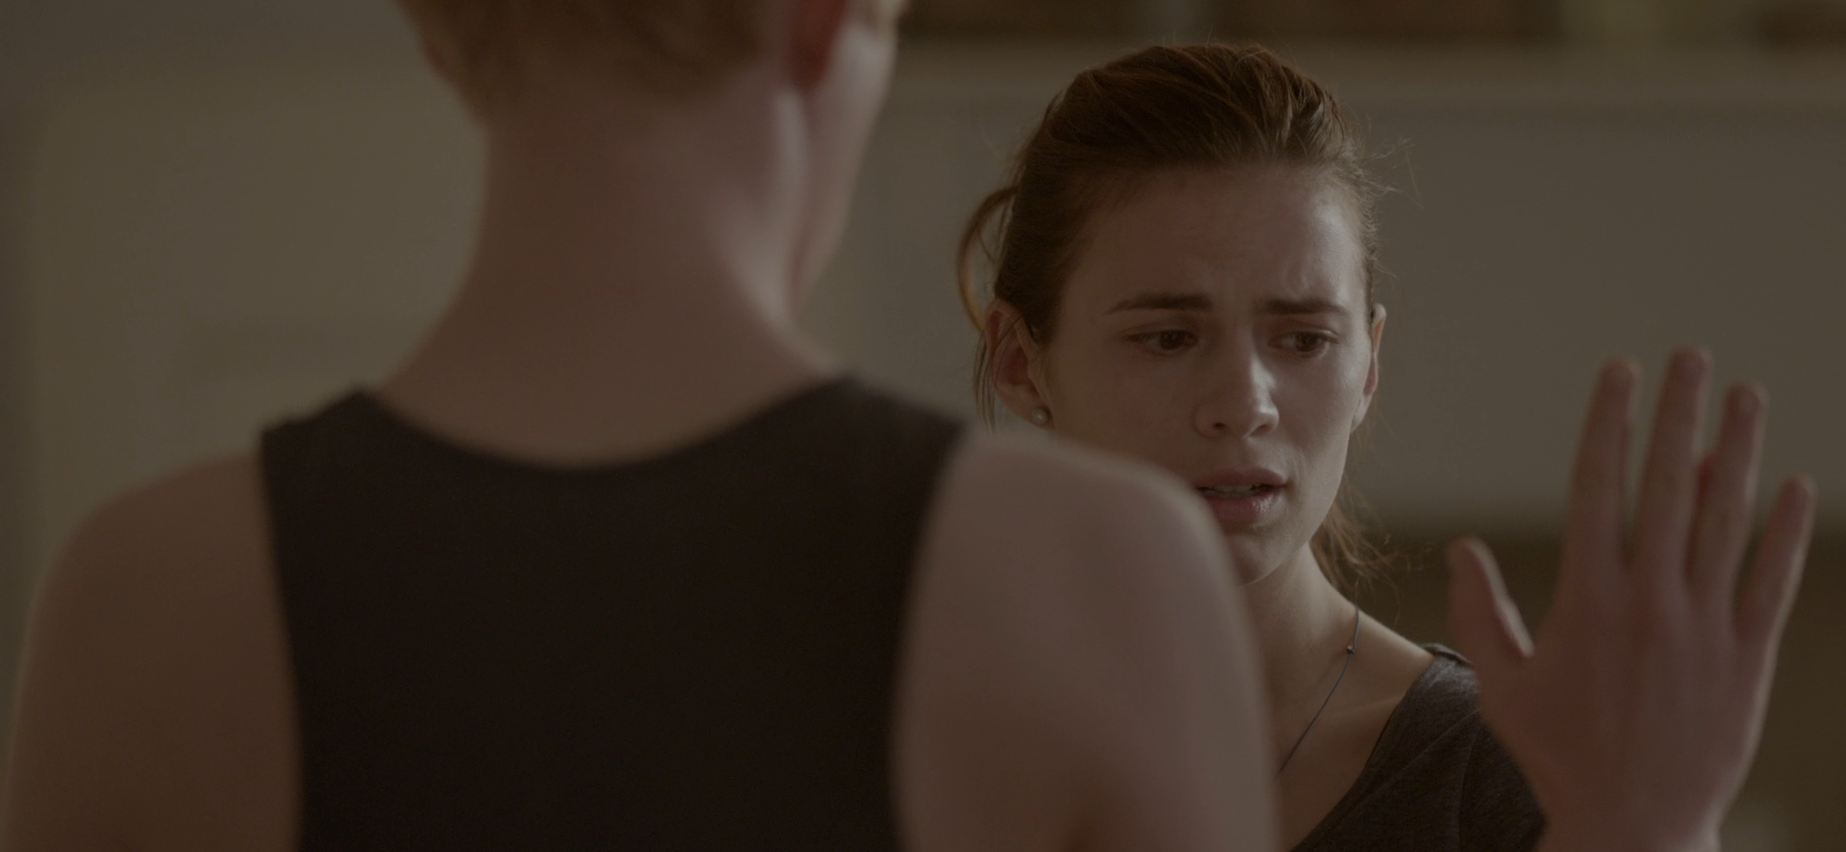
\includegraphics[width=\linewidth,height=.43\textheight,keepaspectratio]{assets/berightback.png}\end{center}
\begin{taskbox}
\tasktitle{Watch}
\begin{enumerate}
\item Watch the episode "Be Right Back" from season 2 of the tv-show Black Mirror
\end{enumerate}
\end{taskbox}

\section*{Working with the text}
\begin{taskbox}
\tasktitle{Create}
\begin{enumerate}
\item In groups, select and analyse a scene from the film that you particularly liked, found important or were intrigued by. In your analysis, you must include a focus on filmic devices such as close-ups, perspective, sound effects or lighting. Moreover, connect the scene to the episode as a whole and give reasons why you picked this scene. Create a slideshow with stills from the film, that presents your analysis.
\end{enumerate}
\end{taskbox}

\section*{Written assignment}
\begin{taskbox}
\tasktitle{Write}
\begin{enumerate}
\item Read the article "How we feel about robots that feel"
\item Write an e-mail from Martha to the company that produced ‘Ash’. Your letter must try to pinpoint what it is that makes a human-robot relationship like this creepy. Be as specific as possible. You can either argue that the company ought to put an end to production or that the company needs to advertise the robots differently. Use formal language (500 words).
\end{enumerate}
\end{taskbox}

\section*{Materials}

\begin{itemize}
\item Black Mirror, S02E01
\item How We Feel About Robots That Feel
\end{itemize}

\clearpage\markboth{Space Policy}{}
\addcontentsline{toc}{chapter}{6. Space Policy}
{\color{blue}\small LESSON 06 \hfill 12 November 2026\par}
\vspace{4mm}
{\displayfont\color{navy}\fontsize{30}{34}\selectfont Space Policy\par}\vspace{4mm}

\section*{Program}

\begin{itemize}
\item \emph{08.35} American values
\item \emph{09.00} On US Space Policy
\item \emph{09.40} Break
\item \emph{09.55} Analysis
\item \emph{10.40} Break
\item \emph{10.50} Sum up
\end{itemize}

\section*{American Values}
\begin{taskbox}
\tasktitle{Research}
\begin{enumerate}
\item Look up information on the following concepts and events in American history. Post small descriptions as well as pictures to illustrate them on edaptio.

\begin{itemize}
\item The Lewis and Clark expedition
\item The pioneers/settlers who went west
\item The frontier thesis
\item Manifest Destiny
\end{itemize}

\end{enumerate}
\end{taskbox}

\begin{center}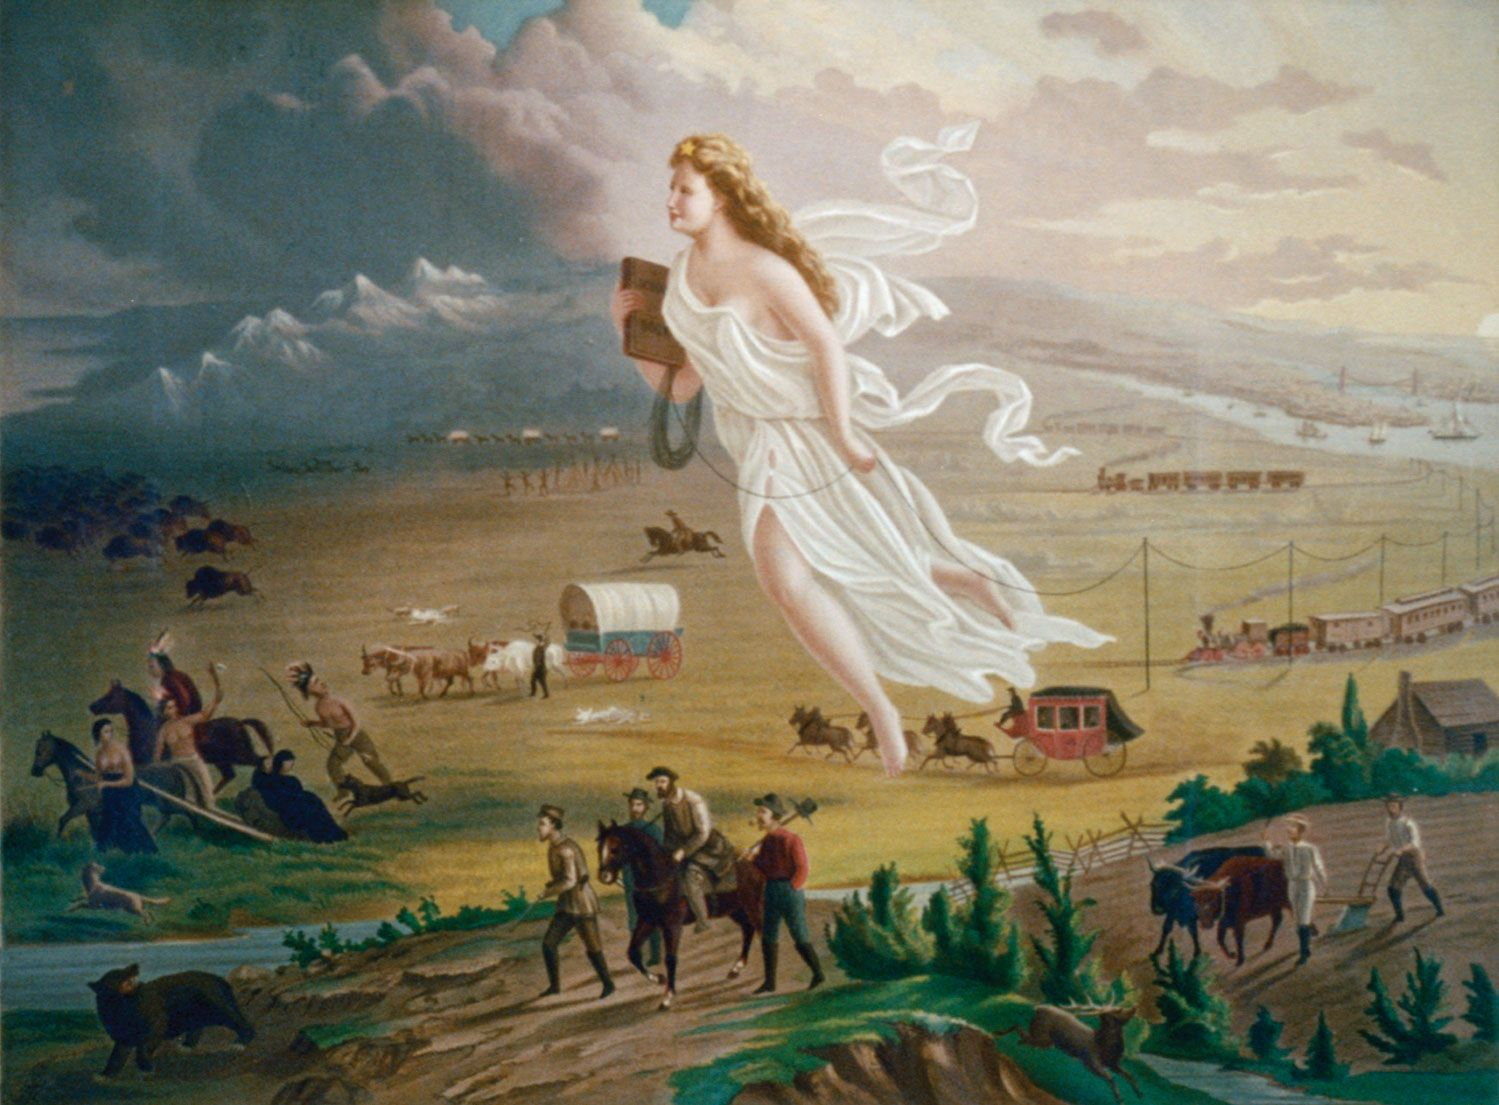
\includegraphics[width=\linewidth,height=.43\textheight,keepaspectratio]{assets/1794426155-manifest.png}\end{center}

\section*{On US Space Policy}
\begin{taskbox}
\tasktitle{Reading focus}
\begin{enumerate}
\item Make notes on the points below and note down the line numbers for the quotes you find interesting and relevant for your focus.

\begin{itemize}
\item Compile a list of rhetorical devices used in the speech.
\item Note down references to American history and values as well as references to mankind in general and international cooperation.
\item Jot down all references to journeys, knowledge and progress.
\item Make a timeline of the milestones proposed by Bush.
\end{itemize}

\end{enumerate}
\end{taskbox}

\section*{Analysis}
\begin{taskbox}
\tasktitle{Discuss}
\begin{enumerate}
\item Discuss answers to questions on hand-out.
\end{enumerate}
\end{taskbox}

\section*{Materials}

\begin{itemize}
\item Remarks on US Space Policy
\item \hyperref[worksheet-4]{Worksheet (p.~\pageref*{worksheet-4})}
\end{itemize}

\clearpage\markboth{Settled In}{}
\addcontentsline{toc}{chapter}{7. Settled In}
{\color{blue}\small LESSON 07 \hfill 16 November 2026\par}
\vspace{4mm}
{\displayfont\color{navy}\fontsize{30}{34}\selectfont Settled In\par}\vspace{4mm}

\section*{Program}

\begin{itemize}
\item \emph{12.05} Warm up
\item \emph{12.25} Settled In
\item \emph{12.50} Break
\item \emph{13.05} Comprehension
\item \emph{13.20} Analysis
\item \emph{14.10} Break
\item \emph{14.20} Essay-writing
\end{itemize}

\section*{Warm up}

\par\noindent\textbf{Video:} Elon Musk shares 'tentative' Mars game plan in SpaceX update at Starbase\par\medskip
\begin{taskbox}
\tasktitle{Reflect}
\begin{enumerate}
\item Do you think Musk's vision of human civilisation being a spacefaring civilisation is utopian?
\item Do you think humans will colonise Mars in your lifetime? How does this make you feel?
\end{enumerate}
\end{taskbox}

\section*{Settled In}
Tim Dudenhoefer is a systems engineer working for NASA at the NASA Goddard Space Flight Center. He grew up outside of Pittsburgh, Pennsylvania along the shores of the Allegheny River where he learned to love the outdoors, reading, writing, science fiction and engineering. He has been writing stories since he was a child.

In 2026 NASA invited writers of sci-fi to submit stories about future journeys and the possible terraforming of Mars to a competition. NASA turned their attention to science fiction as they believed that it might help them “look beyond predictable outcomes and identify mitigation approaches for previously unforeseen risks.“ Tim Dudenhoefer’s story is one of the winning entries in the competition.

\begin{taskbox}
\tasktitle{Read}
\begin{enumerate}
\item Read the short story Settled In by Tim Dudenhoefer
\end{enumerate}
\end{taskbox}

\section*{Comprehension}
\begin{taskbox}
\tasktitle{Discuss}
\begin{enumerate}
\item Where are we when the story begins, and who are the people there?
\item Where are they headed?
\item Who and what are Percy and Jo?
\item What is Shackleton?
\item Who was the narrator’s father and what happened to him?
\item What has happened in the narrator’s personal life since leaving Earth?
\item What role did A.I. play in the human mission to Mars?
\end{enumerate}
\end{taskbox}

\section*{Analysis}
\begin{taskbox}
\tasktitle{Write}
\begin{enumerate}
\item Choose 5 questions on the hand out. Answer each question in writing (at least 50 words).
\item Collect your answers into one text of 5 paragraphs.
\item Try to make the text as cohesive as possible by adding \href{https://theenglishhandbook.systime.dk/?id=247#c1764}{linking words}, an introduction, and/or a conclusion.
\end{enumerate}
\end{taskbox}

\section*{Materials}

\begin{itemize}
\item Settled In
\item \hyperref[worksheet-5]{Worksheet (p.~\pageref*{worksheet-5})}
\end{itemize}

\clearpage\markboth{On a Sunbeam}{}
\addcontentsline{toc}{chapter}{8. On a Sunbeam}
{\color{blue}\small LESSON 08 \hfill 19 November 2026\par}
\vspace{4mm}
{\displayfont\color{navy}\fontsize{30}{34}\selectfont On a Sunbeam\par}\vspace{4mm}

\section*{Program}

\begin{itemize}
\item \emph{08.35} Warm up
\item \emph{08.45} On a Sunbeam
\item \emph{09.15} Break
\item \emph{09.40} Analysis
\item \emph{10.00} Break
\item \emph{10.30} Extra
\end{itemize}

\section*{Warm up}
\begin{taskbox}
\tasktitle{Quick write}
\begin{enumerate}
\item Picture yourself on your back on a lawn at night looking up at the starlit sky. For a minute write down your feelings and thoughts. You might include or find inspiration in some of the words below.

\begin{itemize}
\item vast – fathomless – infinite – alone – insignificant – depth – staggering – indeterminable – unbounded – cosmic – limitless – prodigious – other-worldly – solitude – eternity – ephemeral
\end{itemize}

\end{enumerate}
\end{taskbox}

\begin{center}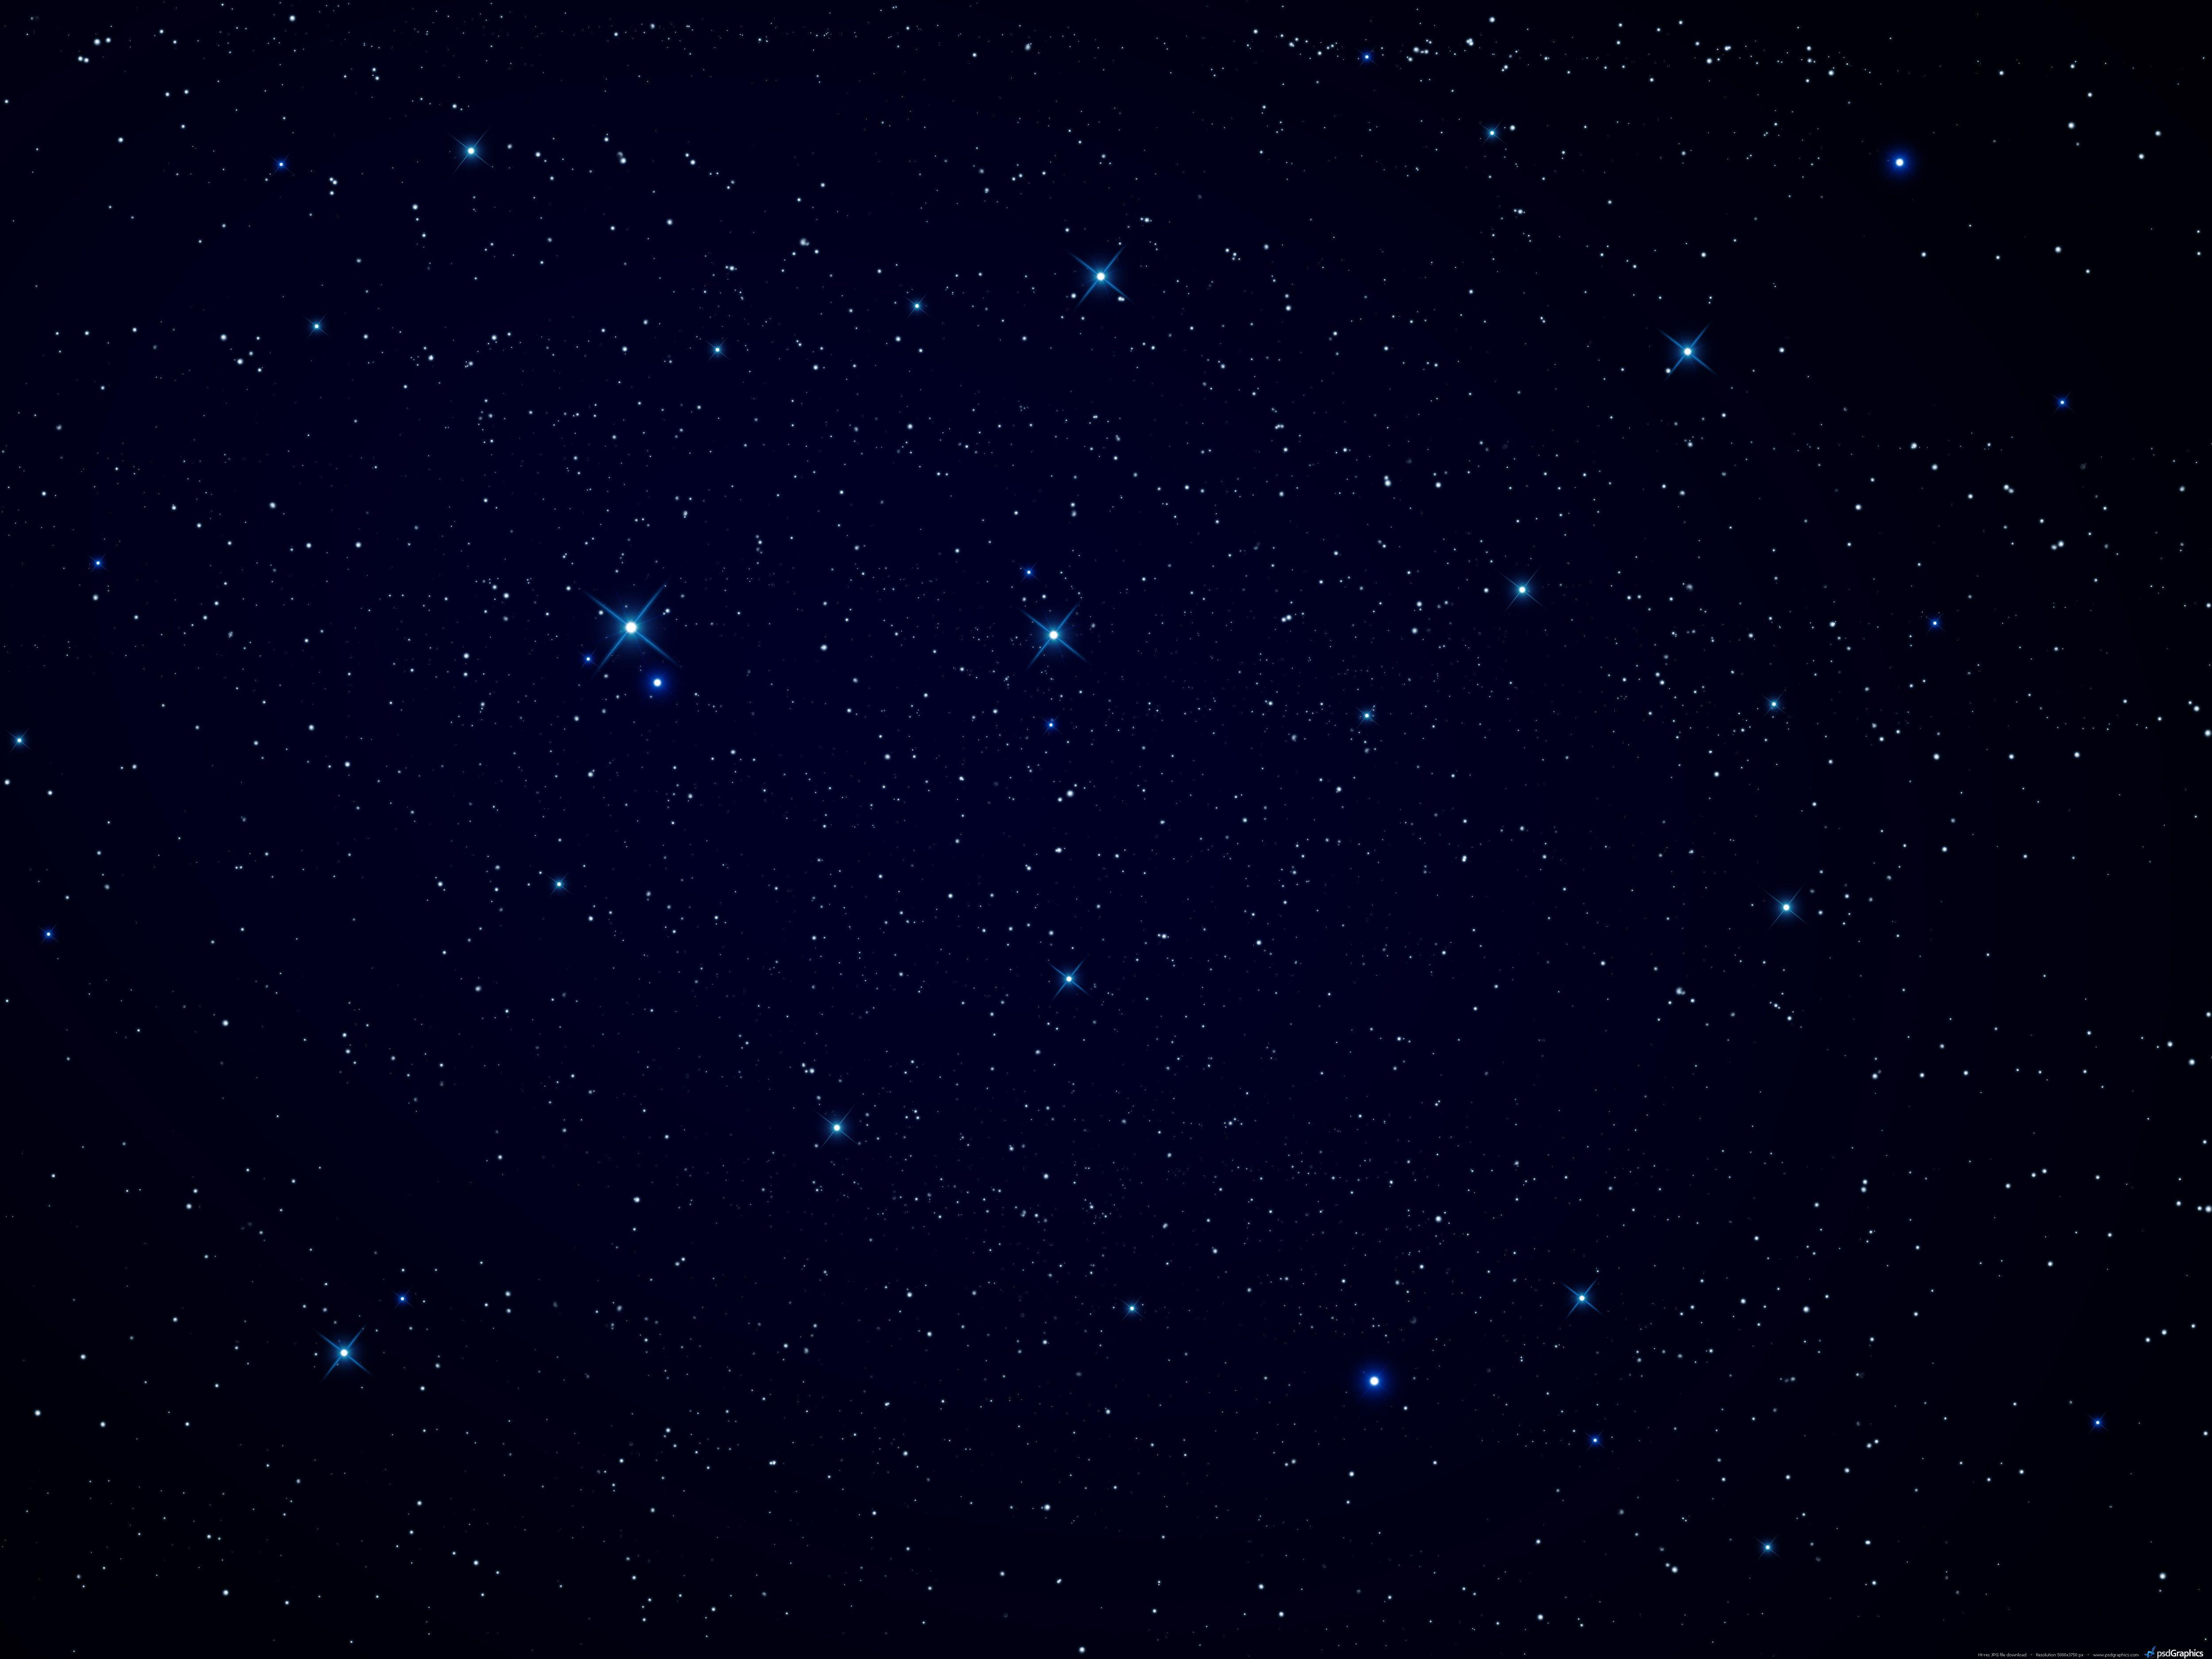
\includegraphics[width=\linewidth,height=.43\textheight,keepaspectratio]{assets/1795013794-sky.png}\end{center}



\section*{On a Sunbeam}

\noindent\begin{minipage}[c]{.51\linewidth}
\begin{taskbox}
\tasktitle{Read}
\begin{enumerate}
\item Read the first two (or three) chapters of the webcomic \href{https://www.onasunbeam.com/}{On a Sunbeam}
\begin{itemize}
\item Pay close attention to the shifting backgrounds.
\item Note the facial expressions and body language of the characters.
\end{itemize}

\end{enumerate}
\end{taskbox}
\end{minipage}\hfill\begin{minipage}[c]{.44\linewidth}\centering
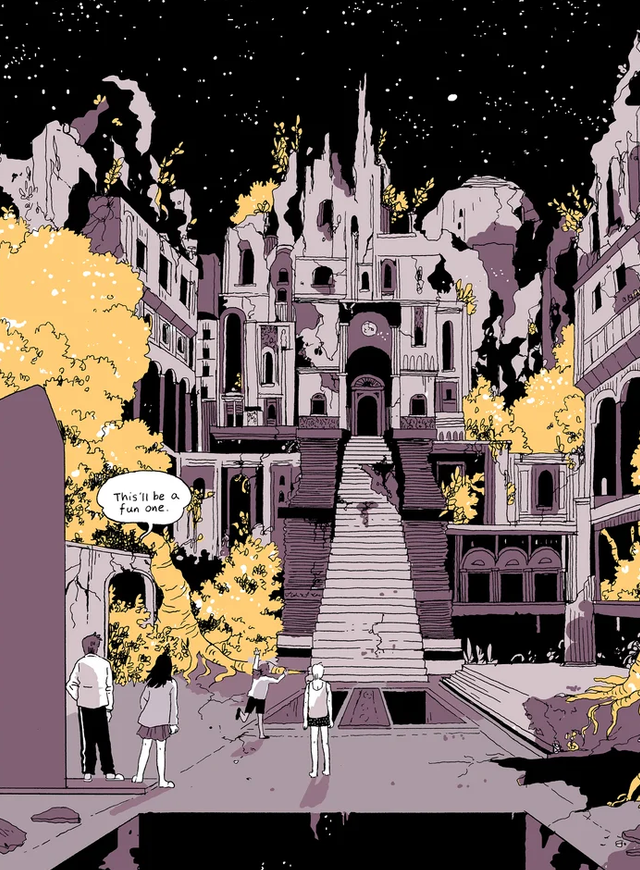
\includegraphics[width=\linewidth,height=.47\textheight,keepaspectratio]{assets/1795014338-sunbeam.png}\end{minipage}\par\medskip

\par\medskip{\color{rule}\hrule}\medskip
\begin{taskbox}
\tasktitle{Discuss}
\begin{enumerate}
\item Why did Mia sign up for the job? What did she expect and what did she get?
\item What do we learn about the society that used to exist where Mia and her crew do construction work?
\item What do we learn about Mia’s job?
\item Make a list of the names of the characters with a small description of who they are and how they are related to the other characters.
\end{enumerate}
\end{taskbox}

\section*{Analysis}
\tasktitle{Work with the text}
\begin{taskbox}
\tasktitle{Option A}
\begin{enumerate}
\item Write a manuscript for a presentation of the text. In your presentation of the text you must:

\begin{itemize}
\item sum up the main points of the text
\item relate the text to the theme
\item make an analysis of the theme of the text
\item speak for approx. 6 minutes
\end{itemize}

\end{enumerate}
\end{taskbox}
\begin{taskbox}
\tasktitle{Option B}
\begin{enumerate}
\item Chose a chapter to add captionboxes to.
\item Find at least 5 panels to write a caption box to. One of your panels must be a silent panel.
\item Take screenshots of the panels and add the boxes to the panels using e.g. canva.
\item Discuss with someone who also chose this option what and if your narrative voice adds anything significant to the story.
\end{enumerate}
\end{taskbox}

\clearpage\markboth{Space Westerns}{}
\addcontentsline{toc}{chapter}{9. Space Westerns}
{\color{blue}\small LESSON 09 \hfill 23 November 2026\par}
\vspace{4mm}
{\displayfont\color{navy}\fontsize{30}{34}\selectfont Space Westerns\par}\vspace{4mm}

\section*{Program}

\begin{itemize}
\item \emph{12.05} Westerns
\item \emph{12.15} The Lone Ranger
\item \emph{12.25} The Mandalorian
\item \emph{13.10} Break
\item \emph{13.25} Analysis
\item \emph{14.25} Break
\item \emph{14.35} Sum up
\end{itemize}

\section*{Westerns}
\begin{taskbox}
\tasktitle{Discuss}
\begin{enumerate}
\item What do you know about the film genre "westerns"?
\item Which movies have you watched / heard about / know the plot of?
\end{enumerate}
\end{taskbox}

\section*{The Lone Ranger}

\noindent\begin{minipage}[c]{.51\linewidth}
\begin{taskbox}
\tasktitle{Research}
\begin{enumerate}
\item Read about The Lone Ranger on wikipedia: How is he characterised?
\end{enumerate}
\end{taskbox}
\end{minipage}\hfill\begin{minipage}[c]{.44\linewidth}\centering
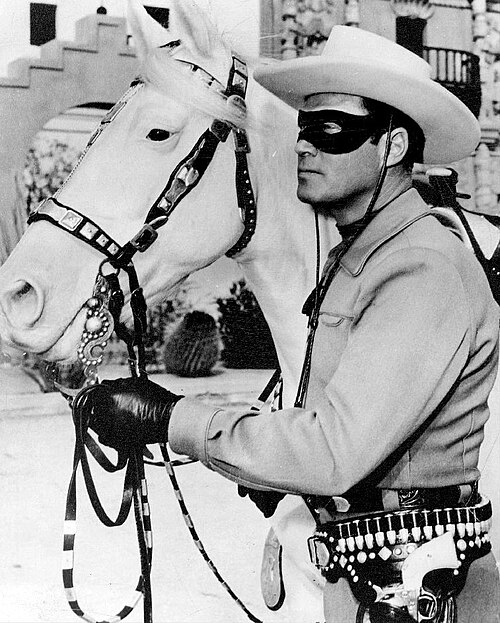
\includegraphics[width=\linewidth,height=.47\textheight,keepaspectratio]{assets/1795372840-loneranger.png}\end{minipage}\par\medskip

\section*{The Mandalorian}

\noindent\begin{minipage}[c]{.51\linewidth}
\begin{taskbox}
\tasktitle{Watch}
\begin{enumerate}
\item Watch the first episode of the tv-series The Mandalorian.
\end{enumerate}
\end{taskbox}
\end{minipage}\hfill\begin{minipage}[c]{.44\linewidth}\centering

\includegraphics[width=\linewidth,height=.47\textheight,keepaspectratio]{assets/1795372963-mando.png}\end{minipage}\par\medskip

\section*{Analysis}
\begin{taskbox}
\tasktitle{Analyse}
\begin{enumerate}
\item Use \href{run:../../../classnotes/eng-c/notes/how-to-analyse.md}{this guide} to analyse the episode. Use only the parts of the guide you find relevant and interesting. Use what you know about western movies and The Lone Ranger in your analysis.
\end{enumerate}
\end{taskbox}

\clearpage\phantomsection\addcontentsline{toc}{chapter}{Worksheets}\markboth{Worksheets}{}
{\displayfont\color{navy}\fontsize{30}{34}\selectfont Worksheets\par}\vspace{6mm}
All worksheets referenced in the lessons are collected below. Click a title or page number to jump to the worksheet.\par
\begin{enumerate}
\item \hyperref[worksheet-1]{Brave New World — Worksheet} \hfill \hyperref[worksheet-1]{p.~\pageref*{worksheet-1}}
\item \hyperref[worksheet-2]{Brave New World II — Worksheet} \hfill \hyperref[worksheet-2]{p.~\pageref*{worksheet-2}}
\item \hyperref[worksheet-3]{The Relive Box — Worksheet} \hfill \hyperref[worksheet-3]{p.~\pageref*{worksheet-3}}
\item \hyperref[worksheet-4]{US Space Policy — Worksheet} \hfill \hyperref[worksheet-4]{p.~\pageref*{worksheet-4}}
\item \hyperref[worksheet-5]{Settled In — Worksheet} \hfill \hyperref[worksheet-5]{p.~\pageref*{worksheet-5}}
\end{enumerate}

\clearpage\markboth{Brave New World — Worksheet}{}
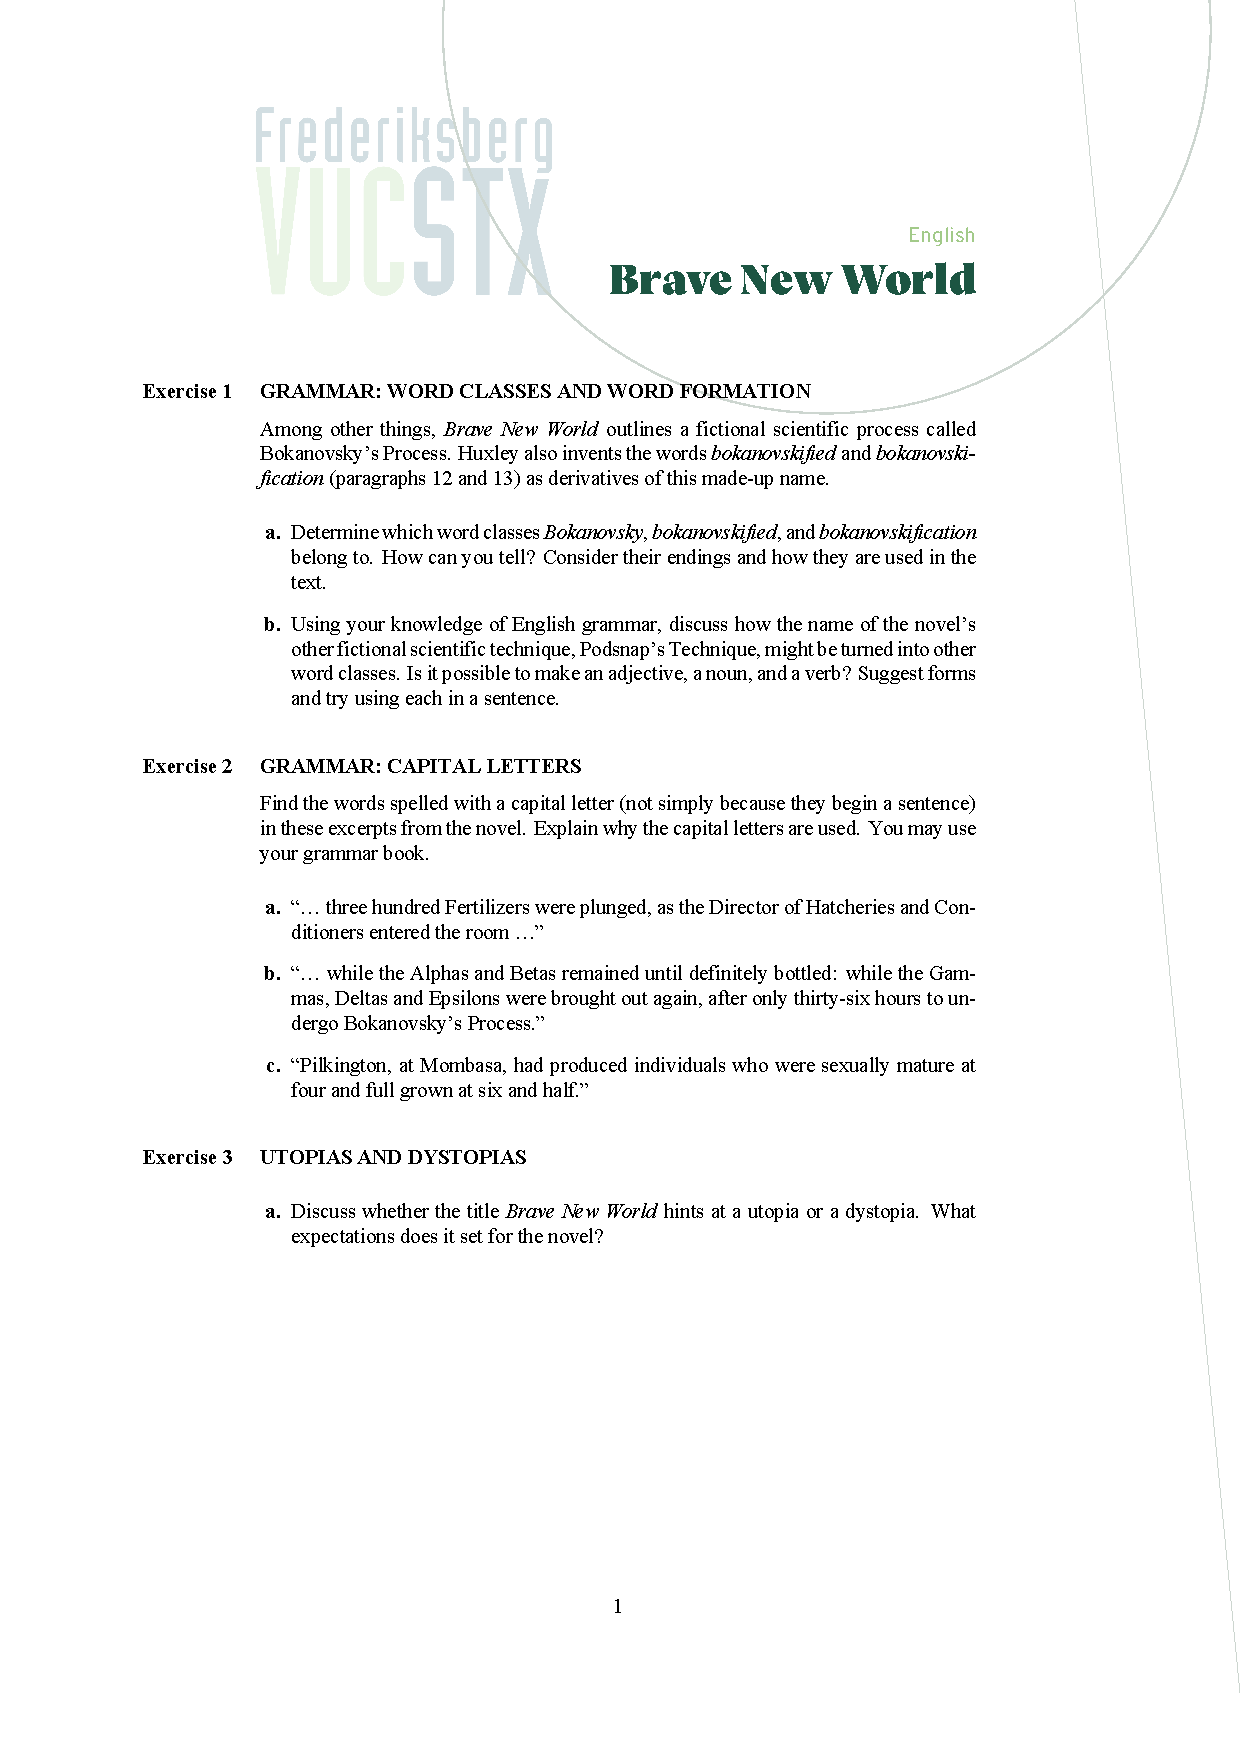
\includepdf[pages=-,scale=.9,pagecommand={\thispagestyle{fancy}},addtotoc={1,section,1,{Brave New World — Worksheet},worksheet-1}]{materials/Brave_New_World_Worksheet.pdf}

\clearpage\markboth{Brave New World II — Worksheet}{}
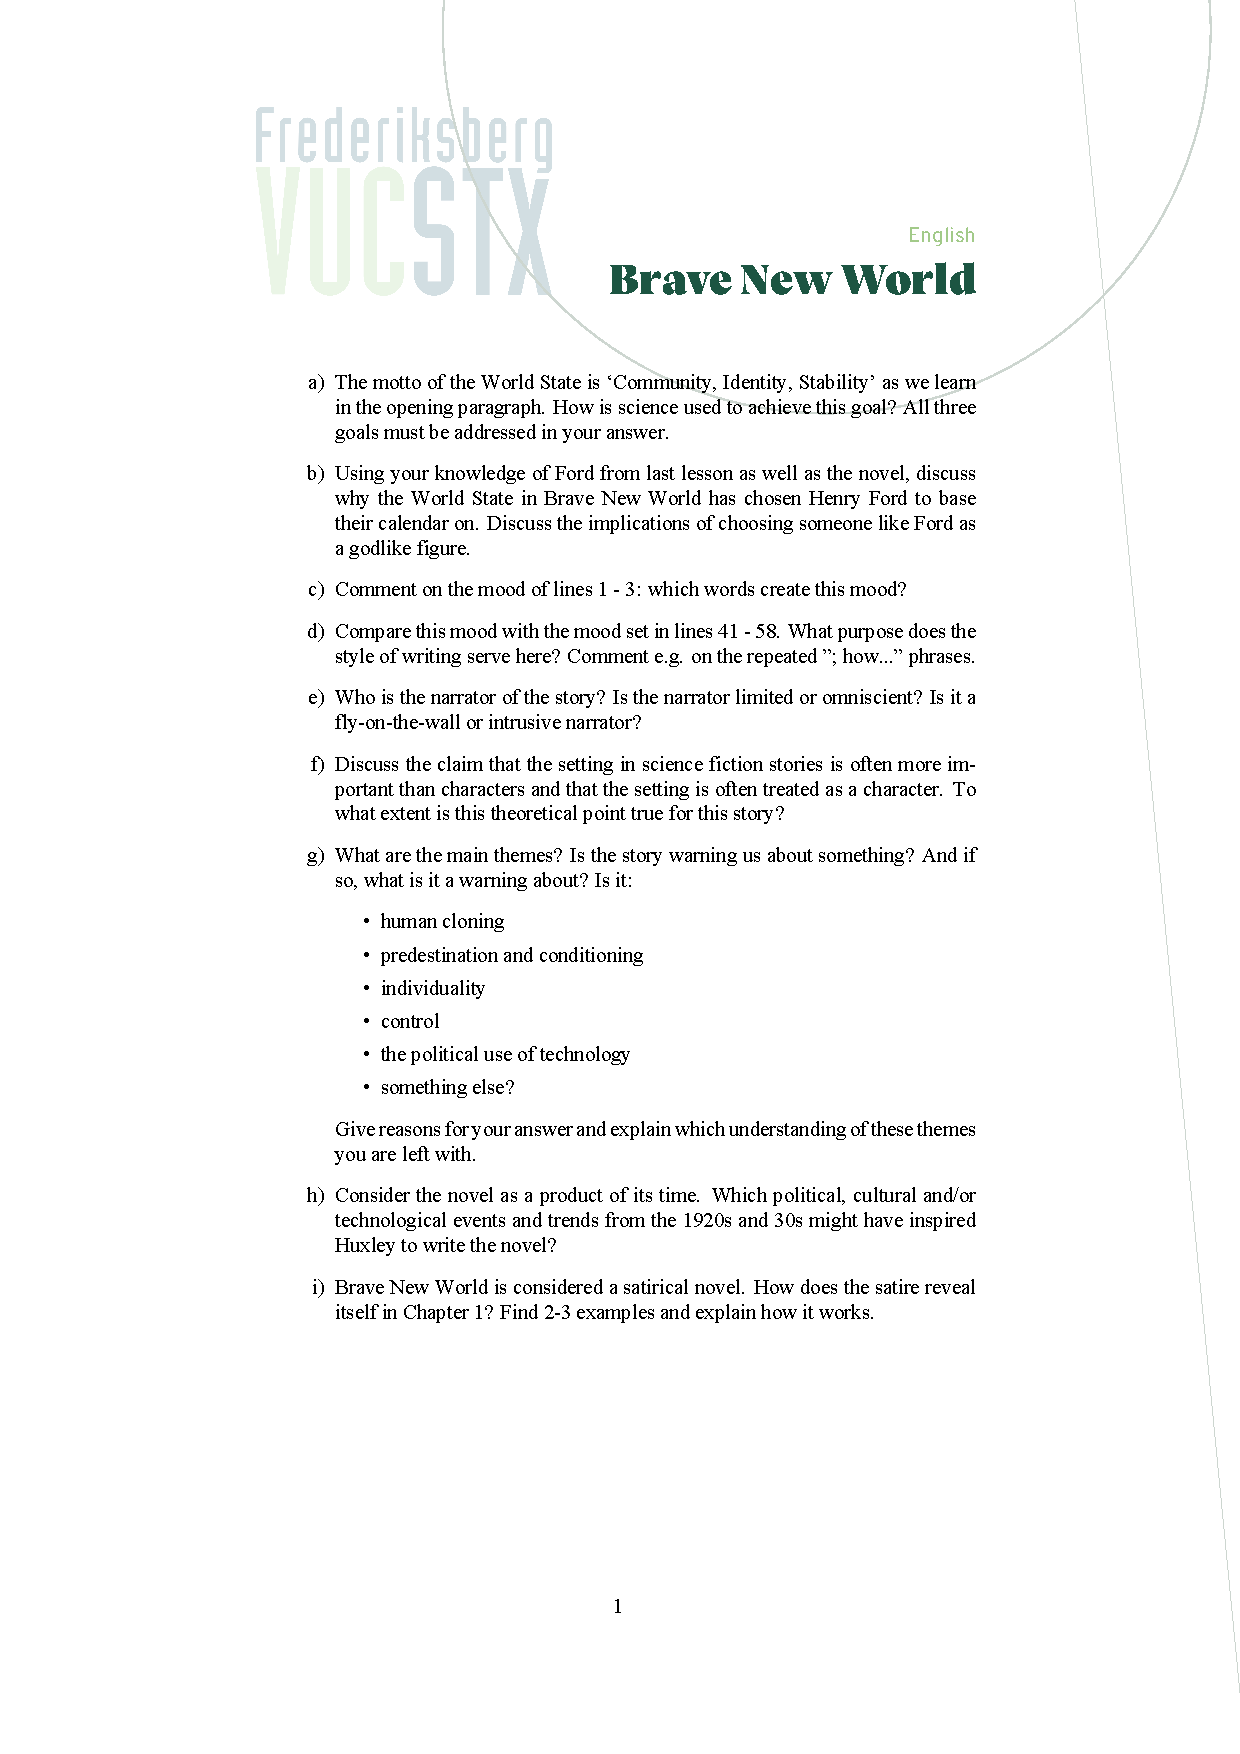
\includepdf[pages=-,scale=.9,pagecommand={\thispagestyle{fancy}},addtotoc={1,section,1,{Brave New World II — Worksheet},worksheet-2}]{materials/Brave_New_World_II_Worksheet.pdf}

\clearpage\markboth{The Relive Box — Worksheet}{}
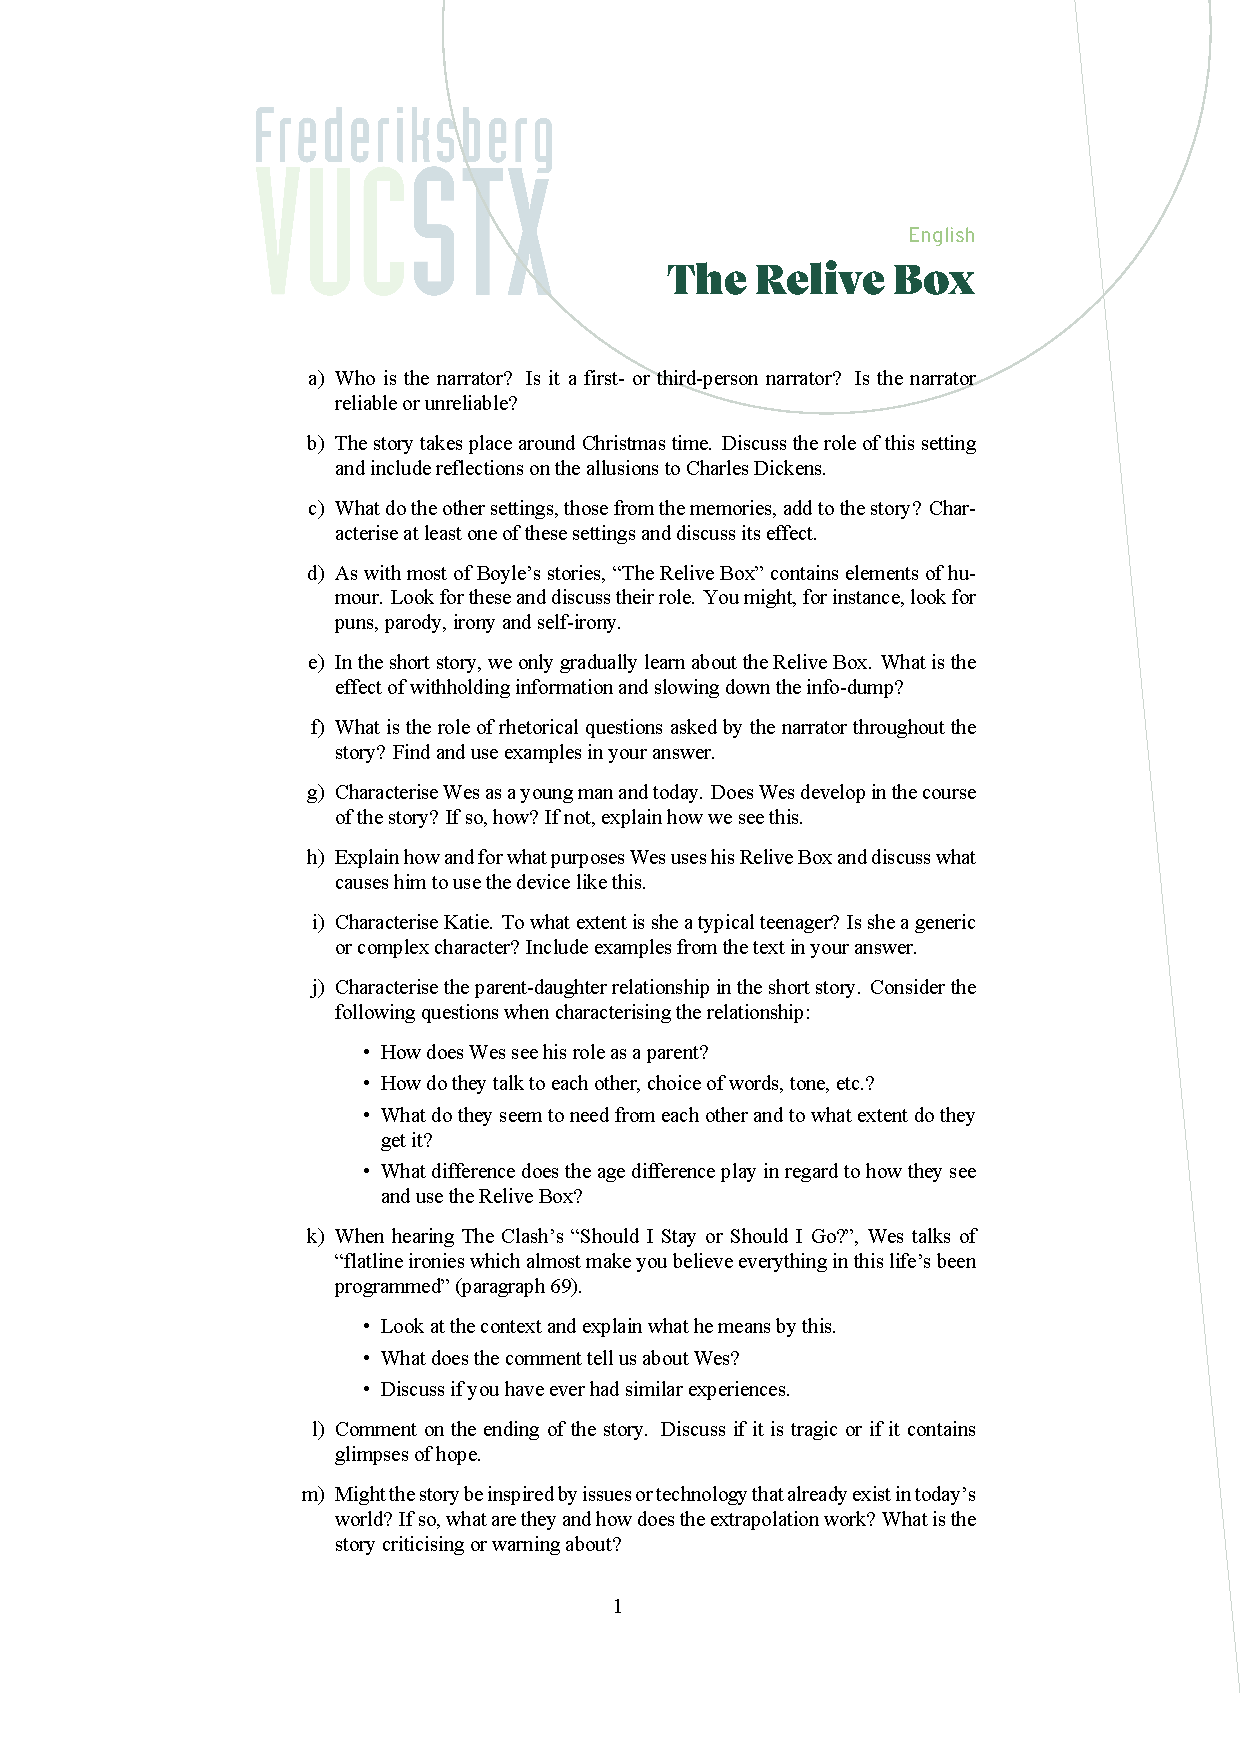
\includepdf[pages=-,scale=.9,pagecommand={\thispagestyle{fancy}},addtotoc={1,section,1,{The Relive Box — Worksheet},worksheet-3}]{materials/The_Relive_Box_Worksheet.pdf}

\clearpage\markboth{US Space Policy — Worksheet}{}
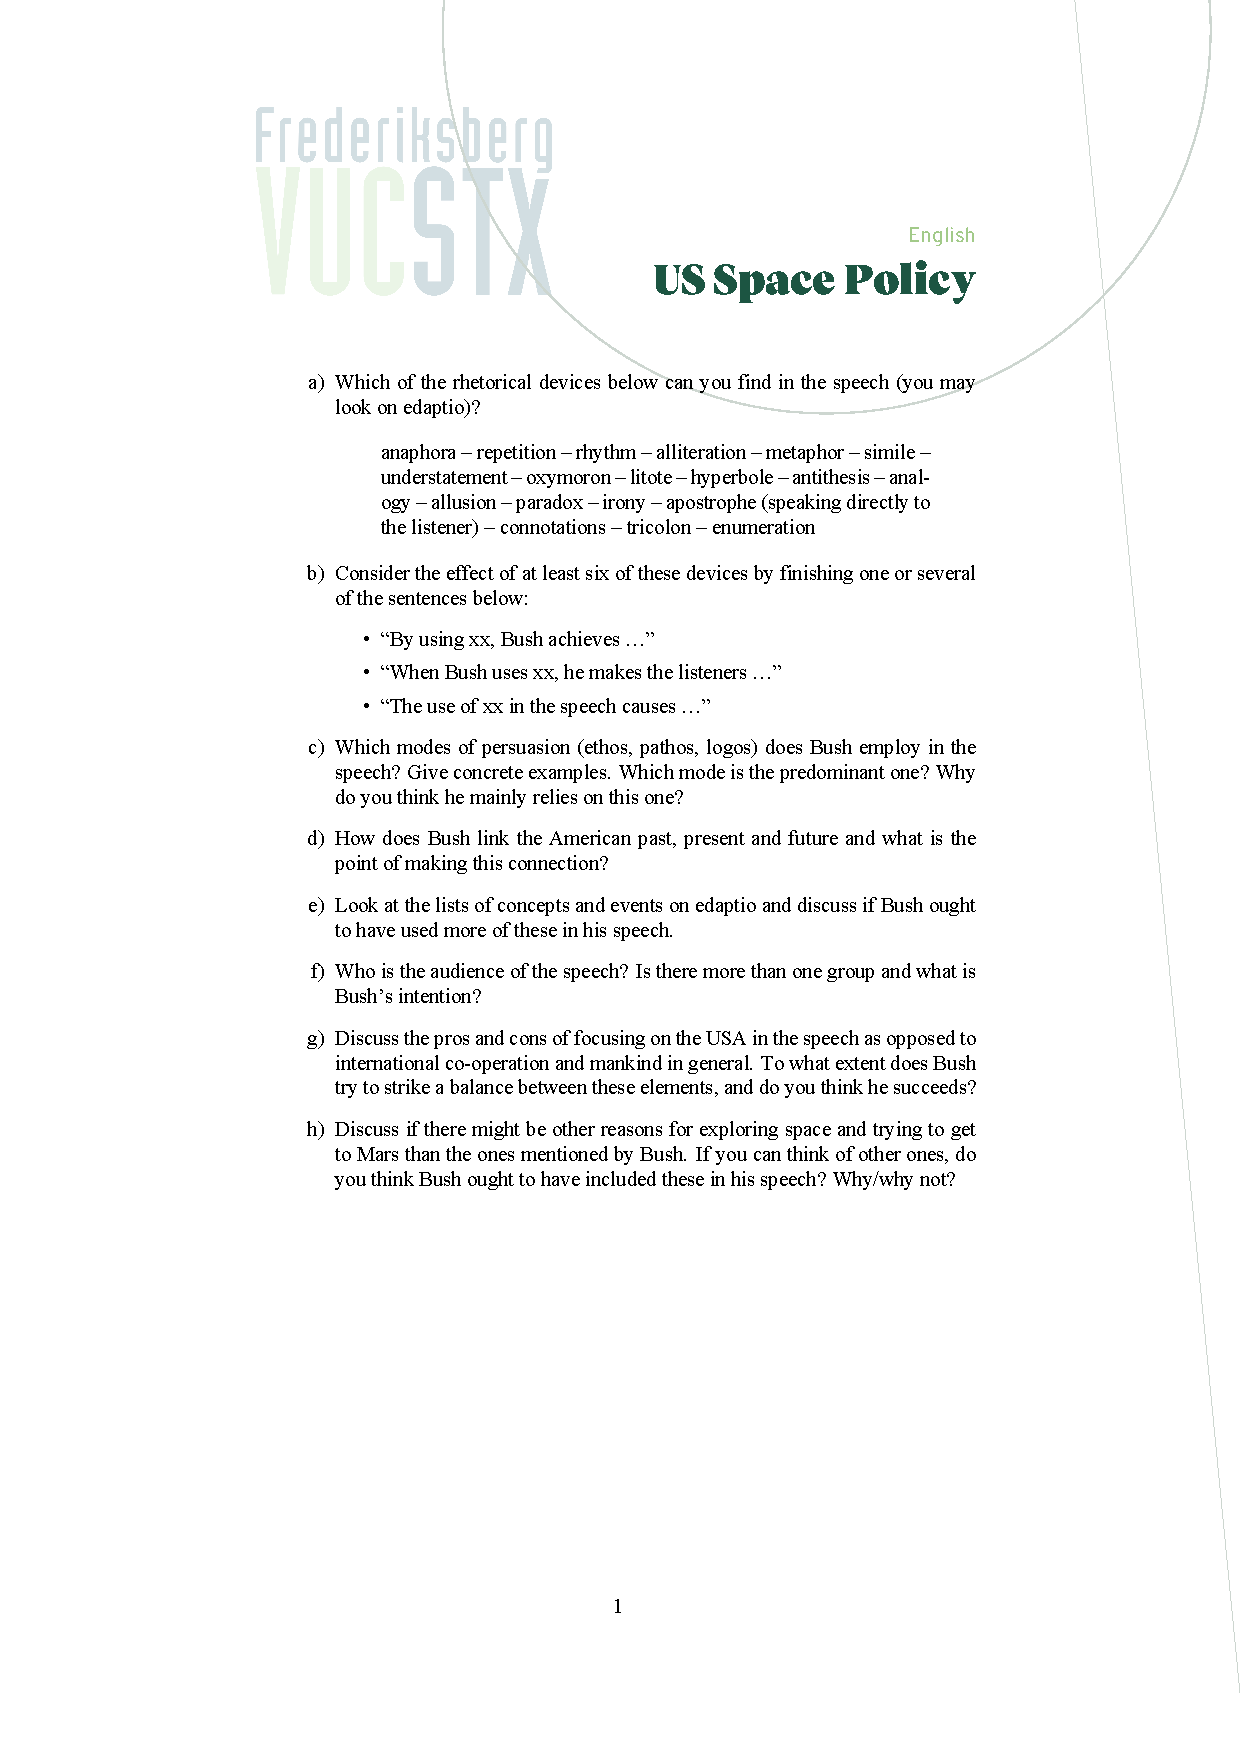
\includepdf[pages=-,scale=.9,pagecommand={\thispagestyle{fancy}},addtotoc={1,section,1,{US Space Policy — Worksheet},worksheet-4}]{materials/US_Space_Policy_Worksheet.pdf}

\clearpage\markboth{Settled In — Worksheet}{}
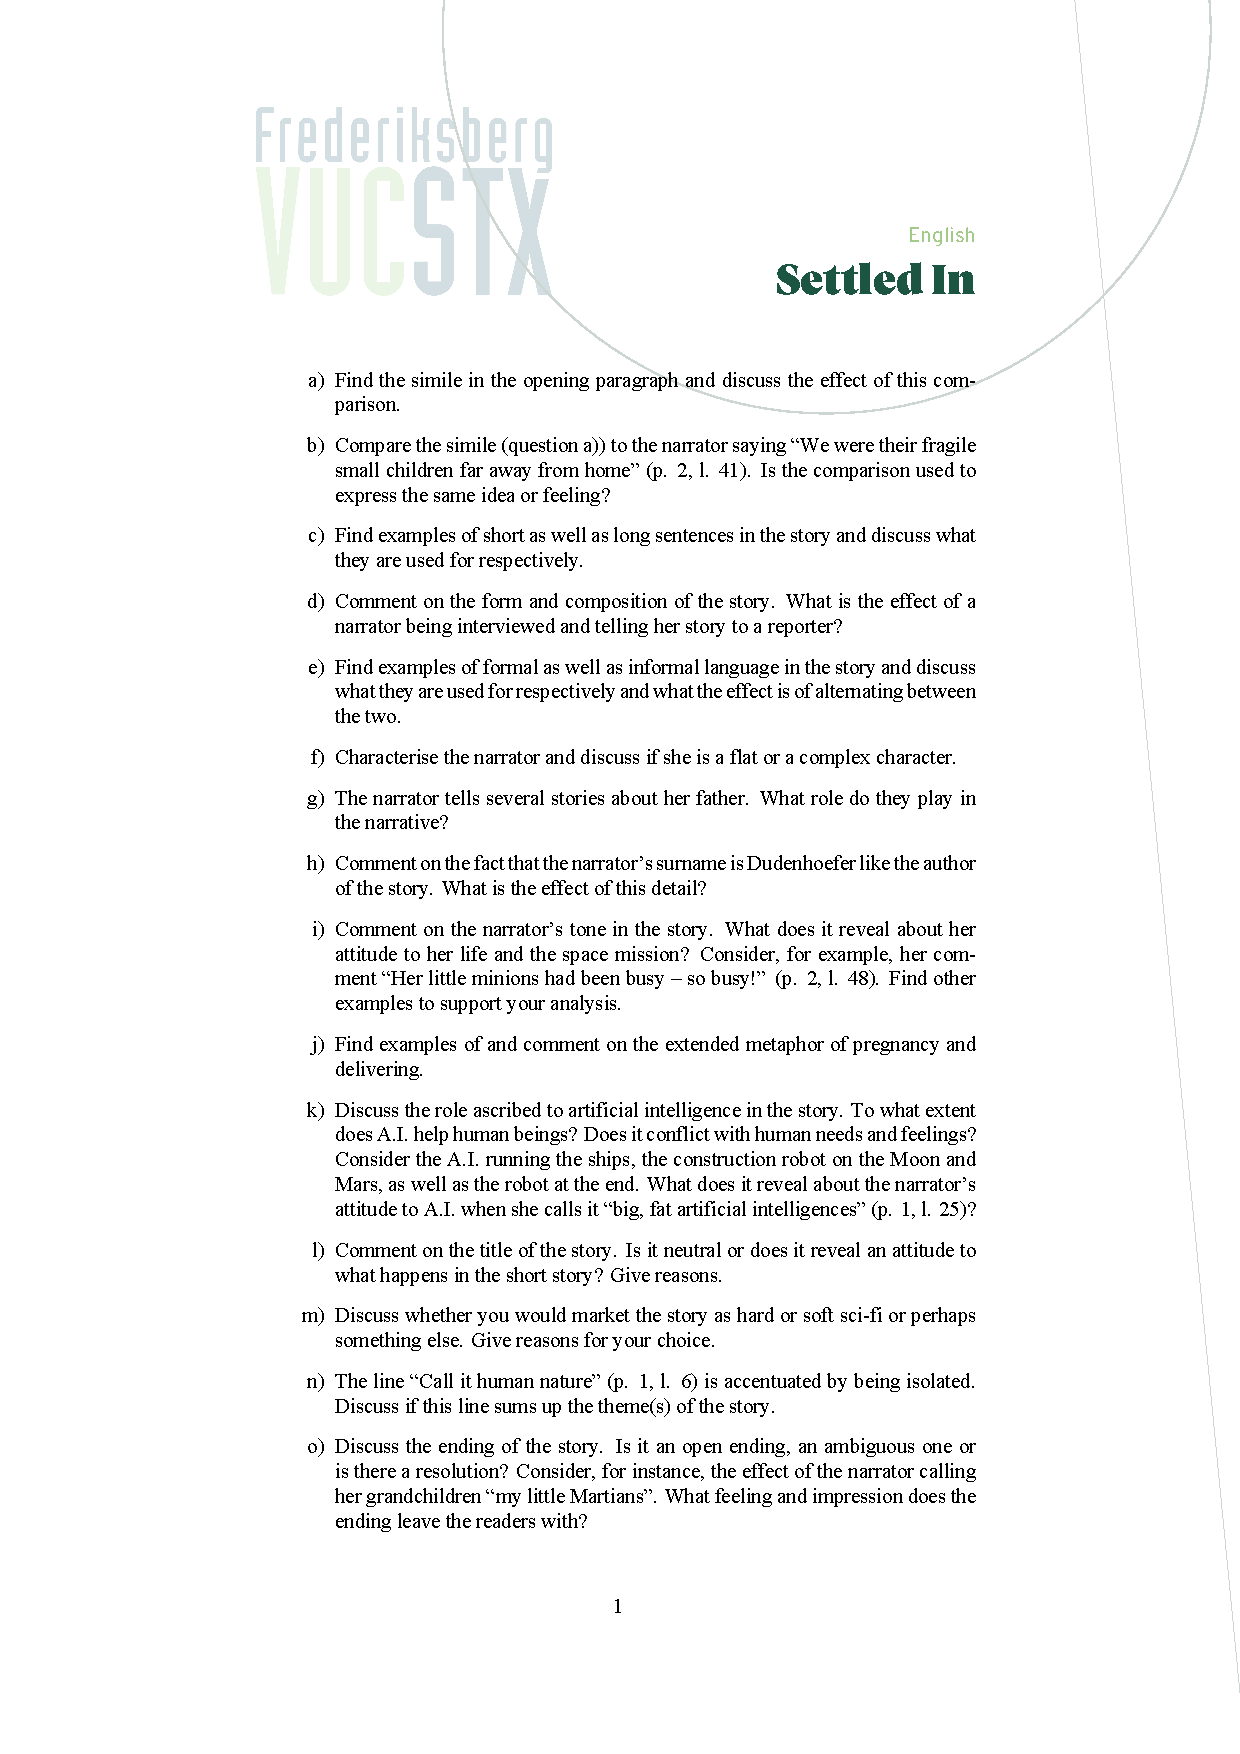
\includepdf[pages=-,scale=.9,pagecommand={\thispagestyle{fancy}},addtotoc={1,section,1,{Settled In — Worksheet},worksheet-5}]{materials/Settled_In_Worksheet.pdf}

\end{document}
